\documentclass[a4paper]{article}
\usepackage[UTF8]{ctex}
\usepackage{amsmath}
\usepackage{enumerate}
\usepackage{tcolorbox}
\usepackage{listings}
\usepackage{graphicx}
\usepackage{fancyhdr}
\usepackage{geometry}
\usepackage{tikz}
\usepackage{harmony}
\usepackage[colorlinks, linkcolor=blue]{hyperref}
\geometry{a4paper, top=2.5cm, bottom=2cm, left=2.5cm, right=2.5cm}

\pagestyle{fancy}
\fancyhf{}
\fancyhead[RE, RO]{\bfseries\thepage}
\fancyhead[L]{\bfseries\leftmark}

\lstset{
	basicstyle=\fontspec{Consolas}
}

\newcommand{\TexMobject}{\texttt{TexMobject}}
\newcommand{\TextMobject}{\texttt{TextMobject}}

\begin{document}

\title{manim 常见问题 v2.1}
\author{鹤翔万里\& catfish}

\maketitle

\newpage



\begin{center}
    \tableofcontents
\end{center} 



\newpage

\begin{center}
    \section{安装问题}
\end{center}
安装时最好不要看 README.md 自己研究。推荐一视数学卷毛杨的两个教程
\begin{itemize}
    \item \url{https://www.bilibili.com/video/av38126904}
    \item \url{https://www.bilibili.com/read/cv4139851}
\end{itemize}

\subsection{Python问题}
\subsubsection*{Q1: 使用anaconda,命令行输入python无反应或报错}

考虑path环境变量是否填全\footnote{安装anaconda时是否勾选添加到path变量},path变量里应该有

\begin{verbatim}
    <your_path>\Anaconda3;
    <your_path>\Anaconda3\Scripts;
    <your_path>\Anaconda3\Library\bin;
\end{verbatim}

\subsubsection*{Q2: pip install ...时满屏红字报错,或者安装过慢}

更换国内镜像源,使用 
\begin{verbatim}
    pip install -r requirements.txt -i https://pypi.tuna.tsinghua.edu.cn/simple
\end{verbatim}

代替\footnote{临时换源}
\begin{verbatim}
    pip install -r requirements.txt
\end{verbatim}

\subsubsection*{Q3: pip安装pycairo总是失败}

下载 pycairo 对应版本的 whl 包\footnote{群文件中有,注意python版本和系统版本是否均合适}
\begin{verbatim}
    pycairo-1.18.2-cp37-cp37m-win_amd64.whl
\end{verbatim}

并手动安装
\begin{verbatim}
    pip install pycairo......whl
\end{verbatim}

\subsubsection*{Q4: pip安装过包,但运行时提示没有模块}
考虑电脑上是否有多个Python,确定pip把包装到了哪个Python上面

\newpage

\begin{center}
    \section{运行时问题}
\end{center}

\subsection{import 问题}
\subsubsection*{Q1: 没有模块\texttt{big\_ol\_pile\_of\_manim\_imports}}

将文件中的
\begin{verbatim}
    from big_ol_pile_of_manim_imports import *
\end{verbatim}

改成
\begin{verbatim}
    from manimlib.imports import *
\end{verbatim}

\subsection{\LaTeX 问题}
\subsubsection*{Q1: 报错Latex error converting to dvi}
先不要管错误在哪,先把manimlib/constants.py中的\texttt{TEX\_USE\_CTEX}改成True再运行

\subsubsection*{Q2: 报错xelatex error converting to xdv}\label{sub:Q2}
若为Windows系统,先把manimlib/constants.py的第29行
\begin{verbatim}
    MEDIA_DIR = "./media"
\end{verbatim}

改成
\begin{verbatim}
    MEDIA_DIR = os.path.join(os.getcwd(), "media")
\end{verbatim}

再进行尝试

\begin{enumerate}[I.]
    \item \textbf{若安装的 \TeX 发行版为 MiK\TeX}
    \begin{enumerate}[1.]
        \item MiK\TeX 的有关路径是否添加到环境变量中
        \item 是否有包没有装全
    \end{enumerate}

    \begin{tcolorbox}
        对于2.,可以正常运行一遍WriteStuff场景,看是否又框弹出提示install什么东西,如果有,则install,并重复运行安装运行安装...直到不报错为止。或者使用tex编辑器(\TeX Studio)并使用xelatex手动编译media/Tex文件夹中的 .tex 文件,查看是否有包没有安装
    \end{tcolorbox}
        
    \begin{tcolorbox}
        对于没有1.、2.问题却依旧报错的,可以选择重新安装新版 MiK\TeX 或者安装 \TeX Live-full 版
    \end{tcolorbox}

    \item \textbf{若安装的 \TeX 发行版为 \TeX Live}
    \begin{enumerate}[1.]
        \item \TeX Live有关路径是否添加到环境变量中
        \item 安装的是否为 full 版本
    \end{enumerate}

    \item \textbf{若安装的 \TeX 发行版不为以上两款}
    
    建议换成 \TeX Live-full 版或者 MiK\TeX,并且在重新安装前请删除旧版
\end{enumerate}

\subsubsection*{Q3: 报错在文件夹内找不到 svg 文件}
清空 media/Tex 文件夹内全部内容,再次运行带文字的场景,查看 Tex 文件夹中的内容

\begin{enumerate}[I.]
    \item 若仅有 tex 文件和 log 文件,按照 \ref{sub:Q2} 中方法处理

    \item 若含有 xdv 文件但没有 svg 文件
    \begin{enumerate}[1.]
        \item divsvgm 是否添加到环境变量,可以使用 \texttt{dvisvgm --version} 观察是否由报错来检查
        \item dvisvgm 版本是否过低,若 \texttt{dvisvgm --verison} 的输出版本号为1开头,请更换新版dvisvgm\footnote{上网下载、或者使用群文件中的版本},并注意将含有 dvisvgm 的文件夹添加到环境变量中
    \end{enumerate}
\end{enumerate}

\subsection{中文显示问题}
\subsubsection*{Q1: 含有中文的 \TextMobject 编译报错 Latex error converting to dvi}

将 manimlib/constants.py 中的 TEX\_USE\_CTEX 改成 True 再尝试

\subsubsection*{Q2: 英文可以正常显示,中文不报错,但不显示}

考虑使用的是否为 \TextMobject 而不是 \TexMobject


\subsection{文字问题}
\subsubsection*{Q1: \TextMobject 和\TexMobject 有什么区别}

\TextMobject 和 \TexMobject 使用的都是 \LaTeX 语法

其中 \TextMobject 文字模式相当于直接在 \LaTeX 环境下书写

\TexMobject 公式模式使用的是 \LaTeX 的 \texttt{\textbackslash begin\{align*\}}
环境或者可以看成加了 \$\$ 的环境

使用 \TextMobject 与 \TexMobject 书写公式时

$$
    \texttt{\TextMobject("}\text{文字}\texttt{\$}\text{公式}\texttt{\$")} \Longleftrightarrow \texttt{\TexMobject("\textbackslash\textbackslash text\{}\text{文字}\texttt{\}}\text{公式}\texttt{")}
$$

\subsubsection*{Q2: \TextMobject 中怎么改字体}

\TextMobject 中只能使用 \LaTeX 的内置字体族和字体形状,包括:
\begin{itemize}
    \item \textrm{罗马字体}   \texttt{\textbackslash textrm\{}\textrm{textrm}\texttt{\}}
    \item \textsf{无衬线字体} \texttt{\textbackslash textsf\{}\textsf{textsf}\texttt{\}}
    \item \texttt{打字机字体} \texttt{\textbackslash texttt\{}\texttt{texttt}\texttt{\}}
    \item \textup{直立形状}   \texttt{\textbackslash textup\{}\textup{textup}\texttt{\}}
    \item \textit{意大利形状} \texttt{\textbackslash textit\{}\textit{textit}\texttt{\}}
    \item \textsl{倾斜形状}   \texttt{\textbackslash textsl\{}\textsl{textsl}\texttt{\}}
    \item \textsc{小型大写}   \texttt{\textbackslash textsc\{}\textsc{textsc}\texttt{\}}
\end{itemize}

\subsubsection*{Q3: 想自定义字体怎么办}

使用新版 manim 特有的 \texttt{Text()} 类,方法如下 \texttt{Text("}文字
\texttt{", font="}字体\texttt{")},其中字体要填写在计算机内存储的格式
\footnote{例如 Microsoft YaHei,Source Han Sans CN},但是不能使用 \LaTeX 语法书写公式

\subsubsection*{Q4: 想用自定义字体写公式怎么办}

可以使用群文件里 cigar666 编写的 \texttt{MyText()} 类$_{\text{Cigar 牛逼}}$

\subsubsection*{Q5: \TexMobject 中换行是什么}
四个右划线 \textbackslash \textbackslash \textbackslash \textbackslash,Python 转义右划线,所以涉及到 \textbackslash{} 的均要写成两个 \textbackslash \textbackslash,而换行在 \LaTeX 中是两个右划线,所以要写成四个\footnote{或者在字符串前加 r,正常书写}

\subsubsection*{Q6: 公式怎么对齐}
\begin{enumerate}[I.]
    \item 直接在 \TexMobject 中使用 \& 对齐
    \item 两个 mobject 对齐,使用 \texttt{obj2.next\_to(obj1, DOWN, aligned\_edge=LEFT)} 使 \texttt{obj2} 在 \texttt{obj1} 下方,并且左对齐
    \item \texttt{VGroup} 内对齐,使用 \texttt{group.arrange(DOWN, aligned\_edge=LEFT)} 使 \texttt{VGroup} 中的子元素依次向下排开,并左对齐
\end{enumerate}

写公式的示例:

\url{https://github.com/Elteoremadebeethoven/AnimationsWithManim/blob/master/English/3_text_like_arrays/scenes.md}

\subsubsection*{Q7: \TexMobject 上色问题的处理办法}
\begin{enumerate}[I.]
    \item 将上色的字符分开,使用 \texttt{text[i].set\_color(color)} 来上色
    \item 将上色的字符分开,使用 \texttt{text.set\_color\_by\_tex\_to\_color\_map(t2c)} 传入 t2c 字典来对相同的字符串上色
    \item 只传入一个字符串,但同时传入 \texttt{tex\_to\_color\_map=t2c} 来自动拆分上色(容易出问题)
    \item 只传入一个字符串,使用 \texttt{text[0][i]} 来对细小的路径上色(一般是一个字符一个下标)
\end{enumerate}

\subsubsection*{Q8: \TexMobject 的下标怎么分析}
创建函数

\begin{lstlisting}
def debugTeX(self, texm):
    for i, j in zip(range(100), texm):
        tex_id = TextMobject(str(i)).scale(0.3).set_color(PURPLE)
        tex_id.move_to(j)
        self.add(tex_id)
\end{lstlisting}

在使用时先 \texttt{self.add(tex)} 然后再 \texttt{debugTeX(self, tex)},导出最后一帧\footnote{-s 选项}\\
观察每段字符上的标号,即为下标

\subsubsection*{Q9: \TexMobject 使用 \texttt{\textbackslash frac} 拆分时出错}
这个是 Grant 写 \texttt{tex\_file\_writing.py} 的一个 bug,建议使用 \{分子 \textbackslash over 分母\} 来代替 \textbackslash frac\{分子\}\{分母\}

\subsection{素材引用问题}

\subsubsection*{Q1: 使用 SVGMobject 找不到 svg 文件}
\begin{enumerate}[I.]
    \item 直接使用绝对路径引用 svg 文件
    \item 将 svg 文件放到 \texttt{assets/svg\_images/} 文件夹中
\end{enumerate}

\subsubsection*{Q2: 如何使用 jpg 或者 png 文件}
\begin{enumerate}[I.]
    \item 直接使用绝对路径引用,并使用 \texttt{ImageMobject}
    \item 将 jpg/png 文件放到 \texttt{assets/raster\_images/} 文件夹中
\end{enumerate}

\newpage

\begin{center}
    \section{其它问题}
\end{center}

\addcontentsline{toc}{subsection}{Q1: 有什么manim教程}

\subsubsection*{Q1: 有什么manim教程}
\begin{enumerate}[1.]
    \item 群主 cigar666 的 B 站专栏
    \begin{itemize}
        \item \url{https://www.bilibili.com/read/readlist/rl82339}
    \end{itemize}
    \item pdcxs 大大转载的 manim 教程
    \begin{itemize}
        \item \url{https://www.bilibili.com/video/av64023740}
        \item 源码\url{https://github.com/Elteoremadebeethoven/AnimationsWithManim}
    \end{itemize}
    \item GitHub 上 cai-hust 的中文教程
    \begin{itemize}
        \item \url{https://github.com/cai-hust/manim-tutorial-CN}
    \end{itemize}
    \item manim 源码
\end{enumerate}

\addcontentsline{toc}{subsection}{Q2: 没有 manim 源码}

\subsubsection*{Q2: 没有 manim 源码}
最好不要使用 \texttt{pip install manimlib} 来装 manim,请在 GitHub 上 clone 下来 manim 的全部内容

\addcontentsline{toc}{subsection}{Q3: 群友用的 manim 都是什么版本}

\subsubsection*{Q3: 群友用的 manim 都是什么版本}
manim 不看版本,一般使用的都是最新版 code。release 里面带版本号的都可以看作旧版

\addcontentsline{toc}{subsection}{Q4: 如何使用傅里叶级数作图}

\subsubsection*{Q4: 如何使用傅里叶级数作图}
套用 Grant 写好的文件
\begin{verbatim}
    active_projects/diffyq/part2/fourier_series.py
    active_projects/diffyq/part4/fourier_series_scenes.py
    active_projects/diffyq/part4/long_fourier_series.py
\end{verbatim}

只需要更换 svg 素材即可(自己制作,或者使用群里的 svg 素材)

\addcontentsline{toc}{subsection}{Q5: svg 用什么软件制作}

\subsubsection*{Q5: svg 用什么软件制作}
Adobe Illustrator(简称 AI) 或者 inkscape(简称 ink)。尽量不要使用网页版编辑器

\addcontentsline{toc}{subsection}{Q6: 一些比较复杂,操纵东西比较多的动画怎么做}

\subsubsection*{Q6: 一些比较复杂,操纵东西比较多的动画怎么做}
使用外部剪辑软件,例如 Adobe Premiere Pro 或者达芬奇

\addcontentsline{toc}{subsection}{Q7: 一个\texttt{self.play}里写两个\texttt{ApplyMethod}只对一个起作用怎么办}

\subsubsection*{Q7: 一个\texttt{self.play}里写两个\texttt{ApplyMethod}只对一个起作用怎么办}
去掉\texttt{ApplyMethod}

\addcontentsline{toc}{subsection}{Q8: 动画怎么显示旋转一个物体}

\subsubsection*{Q8: 动画怎么显示旋转一个物体}
使用\texttt{Ratate}和\texttt{Rotating},区别在群文件中有视频

\addcontentsline{toc}{subsection}{Q9: 怎么控制物体移动或者\texttt{Transform}的加速度}

\subsubsection*{Q9: 怎么控制物体移动或者\texttt{Transform}的加速度}
使用\texttt{rate\_func},一些manim中已经定义的在群文件中有视频

\addcontentsline{toc}{subsection}{Q10: 数学符号/公式 用\LaTeX 怎么打}

\subsubsection*{Q10: 数学符号/公式 用\LaTeX 怎么打}
请见\url{https://www.luogu.com.cn/blog/IowaBattleship/latex-gong-shi-tai-quan}

\addcontentsline{toc}{subsection}{Q11: 使用一些特殊 \LaTeX 的外部包}

\subsubsection*{Q11: 使用一些特殊 \LaTeX 的外部包}

\AAcht \AAcht \AAcht \AAcht \AAcht\\
\textbf{如何使用manim画出上面的音符,或怎么使用这些包?}

在manimlib目录下的ctex\_template.tex或者tex\_template.tex文件中添加外部包的名称\footnote{修改\texttt{TEX\_USE\_CTEX}为True的,可以只在\texttt{ctex\_template.tex}中添加}\\
就拿上面的音符为例,因为是在harmony包中的,所以在tex文件中添加 \texttt{\textbackslash usepackage\{harmony\}}\\
然后新建一个py文件,写入代码
\begin{lstlisting}
    from manimlib.imports import *
    class TestHarmony(Scene):
        def construct(self):
            harmony = TextMobject(
                "\\AAcht \\AAcht \\AAcht \\AAcht \\AAcht",
                color=WHITE,
                stroke_width=1,
                stroke_opacity=1,
            )

            self.play(ShowCreation(harmony))
            self.wait()
\end{lstlisting}

运行py文件即可

\addcontentsline{toc}{subsection}{Q12: 使用 \LaTeX 外部包,编译错误或者无显示}

\subsubsection*{Q12: 使用 \LaTeX 外部包,编译错误或者无显示}
首先,并不是所有外部包都能在manim中顺利使用,大多都不支持xelatex编译,所以建议需要使用外部包时只用latex编译
\footnote{即把\texttt{TEX\_USE\_CTEX}改为True}

至于有些群友常用TiKz这个外部包,也是使用latex才能编译,在xelatex用 \texttt{\textbackslash draw}会无法显示

需要修改\texttt{tex\_template.tex}文件,修改成如下:
\begin{lstlisting}
    \documentclass[preview, dvisvgm]{standalone}
\end{lstlisting}

新建py文件,写入代码

\begin{lstlisting}
    class TestTikz(Scene):
        def construct(self):
            text = TextMobject(
                r"""
                \begin{tikzpicture} 
                    \draw (-1, 0) -- (1, 0); 
                \end{tikzpicture}
                """,
                color=WHITE,
                stroke_width=1,
                stroke_opacity=1,
            )
            self.play(ShowCreation(text))
            self.wait()
\end{lstlisting}

运行py文件即可

\newpage

\subsubsection*{Q13: 如何解决二维画面中的图层问题}
使用z轴坐标对图层进行区分是无效的

可以使用pdcxs添加的\texttt{plot\_depth},具体更改见下图
\begin{figure}[h]
	\begin{center}
		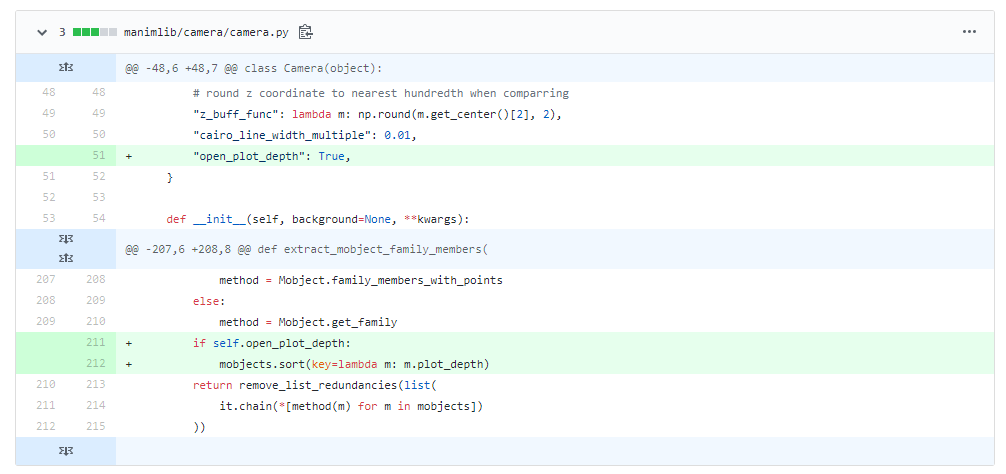
\includegraphics[width=\linewidth]{pd1.png}
	\end{center}
\begin{center}
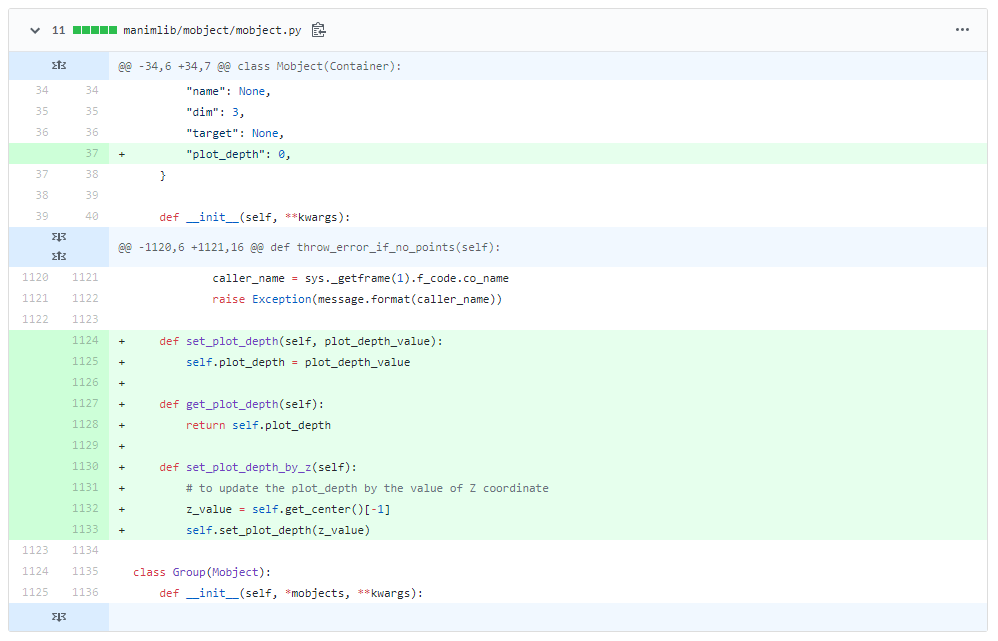
\includegraphics[width=\linewidth]{pd2.png}
\end{center}
\end{figure}

\addcontentsline{toc}{subsection}{Q13: 如何解决二维画面中的图层问题}

\texttt{plot\_depth}的值越大,运行出来的物体就越在上面

\newpage

\addcontentsline{toc}{subsection}{Q14: 如何导出gif文件}

\subsubsection*{Q14: 如何导出gif文件}
在新版本中,manim导出gif已经失效,可以导出mp4,后用ffmpeg转换。也可以按照下图修改源码
\begin{figure}[h]
	\begin{center}
		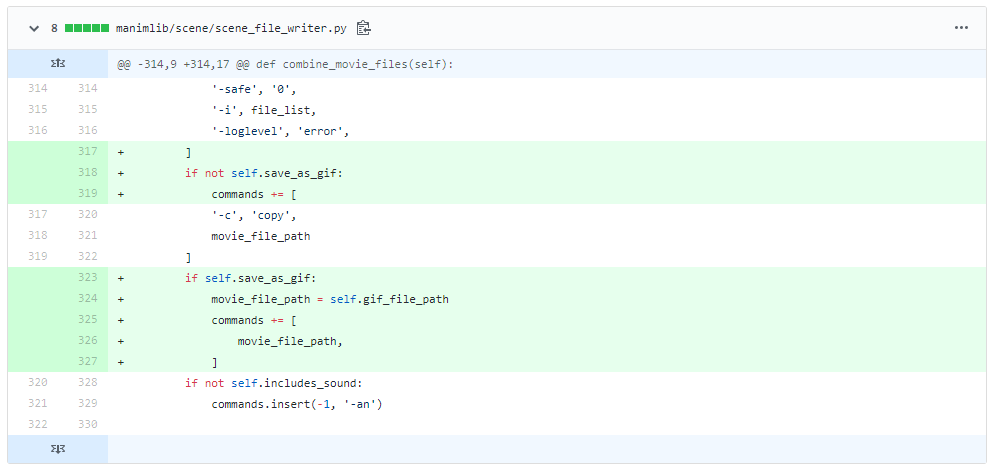
\includegraphics[width=\linewidth]{gif.png}
	\end{center}
\end{figure}

改过后,在输入命令时加上-i选项,就能导出gif了

\addcontentsline{toc}{subsection}{Q15: 如何导出透明的图片或者视频}


\subsubsection*{Q15: 如何导出透明的图片或者视频}
在运行命令的时候加上-t选项
\begin{itemize}
	\item 如果是-s保存图片,则会存储为背景透明的png图片
	\item 如果是-l/-m/-w保存视频,则会存储为背景透明的mov视频文件,方便pr中的剪辑
\end{itemize}

\addcontentsline{toc}{subsection}{Q16: 渲染视频的画质和帧率怎么调整}

\subsubsection*{Q16: 渲染视频的画质和帧率怎么调整}
manim的默认画质有四种
\begin{itemize}
	\item \texttt{-l} 最低画质\ 480P15
	\item \texttt{-m} 中等画质\ 720P30
	\item \texttt{--high\_quality}\footnote{没有缩写} 高画质\ 1080P60
	\item \texttt{-w} 导出(最高)画质\ 1440P60(2K)
\end{itemize}

不加画质选项,默认使用-w最高画质\footnote{比如-p(虽然很多人把-p当成了-w。。。)}。
可以通过修改\texttt{constants.py}中对应的画面长宽和帧率来修改\footnote{manimlib/constants.py的118行开始}

一般把-w最高画质修改成1080P60(B站支持的最高画质)



\subsubsection*{Q17: 有没有什么好的场景例子供学习}

\begin{enumerate}[1.]
	\item Grant的代码\footnote{\texttt{active\_projects}和\texttt{old\_projects}}对应3B1B的视频,可能会有报错,需要魔改
	\item 群文件里“manim相关的python代码及视频结果”
	\item 群里几个B站up主的GitHub库对应他们的代码
	\begin{itemize}
		\item cigar666 \url{https://github.com/cigar666/my_manim_projects}
		\item 鹤翔万里 \url{https://github.com/Tony031218/manim-projects}
		\item pdcxs \url{https://github.com/pdcxs/ManimProjects}
		\item 有一种悲伤叫颓废 \url{https://github.com/136108Haumea/my-manim}\footnote{目前还是空的(颓废.jpg)}
	\end{itemize}
\end{enumerate}

\addcontentsline{toc}{subsection}{Q17: 有没有什么好的场景例子供学习}

\newpage

\begin{center}
    \section{注意}
\end{center}

如果有以上之外的问题,可以在群里提出,或者按照下图操作

    \begin{figure}[h]
        \begin{center}
            \includegraphics[width=6cm]{grant.png}
        \end{center}
    \end{figure}

也请注意群规第 3,4 条
\begin{itemize}
    \item 3.虽为 manim 交流群,但不要一有问题就提出来,简单的问题能自己解决最好,不能解决时再寻求帮助
    \item 4.群主和管理员平时较忙,有时若不能及时回复敬请谅解
\end{itemize}

\end{document}